%
% A header that lets you compile a chapter by itself, or inside a larger document.
% Adapted from http://stackoverflow.com/questions/3655454/conditional-import-in-latex
%
%
%Use \inbpdocument and \outbpdocument in your individual files, in place of \begin{document} and \end{document}. In your main file, put in a \def \ismaindoc {} before including or importing anything.
%
% David Duvenaud
% June 2011
% 
% ======================================
%
%


\ifx\ismaindoc\undefined
	\newcommand{\inbpdocument}{
		\def \ismaindoc {}
		% Use this header if we are compiling by ourselves.
		\documentclass[a4paper,11pt,authoryear,index]{common/PhDThesisPSnPDF}
		
%\usepackage{draftwatermark}
%\SetWatermarkLightness{0.95}

% ******************************************************************************
% ****************************** Custom Margin *********************************

% Add `custommargin' in the document class options to use this section
% Set {innerside margin / outerside margin / topmargin / bottom margin}  and
% other page dimensions

\ifsetMargin
\else
    \RequirePackage[left=37mm,right=30mm,top=35mm,bottom=30mm]{geometry}
    \setFancyHdr % To apply fancy header after geometry package is loaded
\fi


%\chead{Unfinished draft}
%\cfoot{\texttt{Unfinished draft - compiled on \today{} at \currenttime}}

% *****************************************************************************
% ******************* Fonts (like different typewriter fonts etc.)*************

% Add `customfont' in the document class option to use this section

\ifsetFont
\else
    % Set your custom font here and use `customfont' in options. Leave empty to
    % load computer modern font (default LaTeX font).  

    \RequirePackage{libertine} 
\fi

% *****************************************************************************
% *************************** Bibliography  and References ********************

%\usepackage{cleveref} %Referencing without need to explicitly state fig /table

% Add `custombib' in the document class option to use this section
\ifsetBib % True, Bibliography option is chosen in class options
\else % If custom bibliography style chosen then load bibstyle here

   \RequirePackage[square, sort, numbers, authoryear]{natbib} % CustomBib

% If you would like to use biblatex for your reference management, as opposed to the default `natbibpackage` pass the option `custombib` in the document class. Comment out the previous line to make sure you don't load the natbib package. Uncomment the following lines and specify the location of references.bib file

% \RequirePackage[backend=biber, style=numeric-comp, citestyle=numeric, sorting=nty, natbib=true]{biblatex}
% \bibliography{References/references} %Location of references.bib only for biblatex

\fi


% changes the default name `Bibliography` -> `References'
\renewcommand{\bibname}{References}


% *****************************************************************************
% *************** Changing the Visual Style of Chapter Headings ***************
% Uncomment the section below. Requires titlesec package.

%\RequirePackage{titlesec}
%\newcommand{\PreContentTitleFormat}{\titleformat{\chapter}[display]{\scshape\Large}
%{\Large\filleft{\chaptertitlename} \Huge\thechapter}
%{1ex}{}
%[\vspace{1ex}\titlerule]}
%\newcommand{\ContentTitleFormat}{\titleformat{\chapter}[display]{\scshape\huge}
%{\Large\filleft{\chaptertitlename} \Huge\thechapter}{1ex}
%{\titlerule\vspace{1ex}\filright}
%[\vspace{1ex}\titlerule]}
%\newcommand{\PostContentTitleFormat}{\PreContentTitleFormat}
%\PreContentTitleFormat


% *****************************************************************************
% **************************** Custom Packages ********************************
% *****************************************************************************


% ************************* Algorithms and Pseudocode **************************

%\usepackage{algpseudocode} 


% ********************Captions and Hyperreferencing / URL **********************

% Captions: This makes captions of figures use a boldfaced small font. 
%\RequirePackage[small,bf]{caption}

\RequirePackage[labelsep=space,tableposition=top]{caption} 
%\renewcommand{\figurename}{Figure} %to support older versions of captions.sty
\captionsetup{belowskip=12pt,aboveskip=4pt}

% ************************ Formatting / Footnote *******************************

%\usepackage[perpage]{footmisc} %Range of footnote options 


% ****************************** Line Numbers **********************************

%\RequirePackage{lineno}
%\linenumbers

% ************************** Graphics and figures *****************************

%\usepackage{rotating}
%\usepackage{wrapfig}
%\usepackage{float}
\usepackage{subfig} %note: subfig must be included after the `caption` package. 


% ********************************* Table **************************************

%\usepackage{longtable}
%\usepackage{multicol}
%\usepackage{multirow}
%\usepackage{tabularx}


% ***************************** Math and SI Units ******************************

\usepackage{amsfonts}
\usepackage{amsmath}
\usepackage{amssymb}
%\usepackage{siunitx} % use this package module for SI units


% ******************************************************************************
% ************************* User Defined Commands ******************************
% ******************************************************************************

% *********** To change the name of Table of Contents / LOF and LOT ************

%\renewcommand{\contentsname}{My Table of Contents}
%\renewcommand{\listfigurename}{List of figures}
%\renewcommand{\listtablename}{List of tables}


% ********************** TOC depth and numbering depth *************************

\setcounter{secnumdepth}{2}
\setcounter{tocdepth}{2}

% ******************************* Nomenclature *********************************

% To change the name of the Nomenclature section, uncomment the following line

%\renewcommand{\nomname}{Symbols}


% ********************************* Appendix ***********************************

% The default value of both \appendixtocname and \appendixpagename is `Appendices'. These names can all be changed via: 

%\renewcommand{\appendixtocname}{List of appendices}
%\renewcommand{\appendixname}{Appndx}

		% All my custom preamble stuff.  Shouldn't overlap with anything in official-preamble


% Paths to figure and table directories.
\newcommand{\symmetryfigsdir}{figures/symmetries}
\newcommand{\topologyfiguresdir}{figures/topology}
\newcommand{\infinitefiguresdir}{figures/infinite}
\newcommand{\grammarfiguresdir}{figures/grammar}
\newcommand{\introfigsdir}{figures/intro}
\newcommand{\gplvmfiguresdir}{figures/gplvm}
\newcommand{\warpedfiguresdir}{figures/warped-mixtures}
\newcommand{\deeplimitsfiguresdir}{figures/deep-limits}
\newcommand{\quadraturefigsdir}{figures/quadrature}
\newcommand{\additivefigsdir}{figures/additive}
\newcommand{\decompfigsdir}{figures/decomp}
\newcommand{\examplefigsdir}{figures/worked-example}


\usepackage{bm}  % for warped mixtures - is this necessary?
\usepackage{booktabs}
\usepackage{tabularx}
\usepackage{multirow}
\usepackage{datetime}
\renewcommand{\tabularxcolumn}[1]{>{\arraybackslash}m{#1}}
\usepackage{relsize}
\usepackage{graphicx}
\usepackage{amsmath,amssymb,textcomp}
\usepackage{nicefrac}
\usepackage{amsthm}
\usepackage{tikz}
\usetikzlibrary{arrows}
\usetikzlibrary{calc}
\usepackage{nth}
\usepackage{rotating}
\usepackage{array}
\usepackage{fp}
\usepackage[hyperpageref]{backref}
\def\foo{\hspace{\fill}\mbox{}\linebreak[0]\hspace*{\fill}}
\renewcommand*{\backref}[1]{}
\renewcommand*{\backrefalt}[4]{%
\ifcase #1 %
%
\or
\foo(page #2)%
\else
\foo(pages #2)%
\fi
}

\usepackage{cleveref}
\crefname{equation}{equation}{equations}


%% For submission, make all render blank.
%%%%%%%%%%%%%%%%%%%%%%%%%%%%%%%%%%%%%%%%%%%%%%%%%%%%%%%%%%
%%%% EDITING HELPER FUNCTIONS  %%%%%%%%%%%%%%%%%%%%%%%%%%%
%%%%%%%%%%%%%%%%%%%%%%%%%%%%%%%%%%%%%%%%%%%%%%%%%%%%%%%%%%

%% NA: needs attention (rough writing whose correctness needs to be verified)
%% TBD: instructions for how to fix a gap ("Describe the propagation by ...")
%% PROBLEM: bug or missing crucial bit 

%% use \fXXX versions of these macros to put additional explanation into a footnote.  
%% The idea is that we don't want to interrupt the flow of the paper or make it 
%% impossible to read because there are a bunch of comments.

%% NA's (and TBDs, those less crucially) should be written so 
%% that they flow with the text.

\definecolor{WowColor}{rgb}{.75,0,.75}
\definecolor{SubtleColor}{rgb}{0,0,.50}

% inline
\newcommand{\NA}[1]{\textcolor{SubtleColor}{ {\tiny \bf ($\star$)} #1}}
\newcommand{\LATER}[1]{\textcolor{SubtleColor}{ {\tiny \bf ($\dagger$)} #1}}
\newcommand{\TBD}[1]{\textcolor{SubtleColor}{ {\tiny \bf (!)} #1}}
\newcommand{\PROBLEM}[1]{\textcolor{WowColor}{ {\bf (!!)} {\bf #1}}}

% as margin notes

\newcounter{margincounter}
\newcommand{\displaycounter}{{\arabic{margincounter}}}
\newcommand{\incdisplaycounter}{{\stepcounter{margincounter}\arabic{margincounter}}}

\newcommand{\fTBD}[1]{\textcolor{SubtleColor}{$\,^{(\incdisplaycounter)}$}\marginpar{\tiny\textcolor{SubtleColor}{ {\tiny $(\displaycounter)$} #1}}}

\newcommand{\fPROBLEM}[1]{\textcolor{WowColor}{$\,^{((\incdisplaycounter))}$}\marginpar{\tiny\textcolor{WowColor}{ {\bf $\mathbf{((\displaycounter))}$} {\bf #1}}}}

\newcommand{\fLATER}[1]{\textcolor{SubtleColor}{$\,^{(\incdisplaycounter\dagger)}$}\marginpar{\tiny\textcolor{SubtleColor}{ {\tiny $(\displaycounter\dagger)$} #1}}}

%\renewcommand{\LATER}[1]{}
%\renewcommand{\fLATER}[1]{}
%\renewcommand{\TBD}[1]{}
%\renewcommand{\fTBD}[1]{}
%\renewcommand{\PROBLEM}[1]{}
%\renewcommand{\fPROBLEM}[1]{}
%\renewcommand{\NA}[1]{}


% HUMBLE WORDS: shown slightly smaller when in normal text
% Thanks to Christian Steinruecken!

% HUMBLE WORDS: shown slightly smaller when in normal text
%
\makeatletter%
%\def\@humbleformat#1{{\fontsize{}{1em}\selectfont #1}}
%\def\@humbleformat#1{\textsmaller{#1}}%
\newlength{\nonHumbleHeight}
\def\@humbleformat#1{{\settoheight{\nonHumbleHeight}{#1}\resizebox{!}{0.94\nonHumbleHeight}{#1}}}%
\def\@idxhumbleformat#1{{\relscale{0.95}{#1}}}%
%\def\@humbleformat#1{{#1}}%
\def\declareHumble#1#2{%
  \expandafter\def\csname #1\endcsname{\@humbleformat{#2}}%
  \expandafter\def\csname s#1\endcsname{{#2}}%
  \expandafter\def\csname idx#1\endcsname{{\@idxhumbleformat{#2}}}%
}%
\def\humble#1{\@humbleformat{#1}}%
\def\idxhumble#1{\@idxhumbleformat{#1}}%
\makeatother%

% Convenient indexing for humble abbreviations
\def\humbleindex#1#2{\index{#1@\idxhumble{#1}}}



% TODO: Clean up duplicates
\declareHumble{ANOVA}{ANOVA}
\declareHumble{ARD}{ARD}
\declareHumble{BIC}{BIC}
\declareHumble{BMC}{BMC}
\declareHumble{bq}{BQ}
\declareHumble{CRP}{CRP}
\declareHumble{dirpro}{DP}
\declareHumble{HDMR}{HDMR}
\declareHumble{GAM}{GAM}
\declareHumble{GEM}{GEM}
\declareHumble{GMM}{GMM}
\declareHumble{gplvm}{GP-LVM}
\declareHumble{gpml}{GPML}
\declareHumble{GPML}{GPML}
\declareHumble{gprn}{GPRN}
\declareHumble{gpt}{GP}
\declareHumble{gp}{GP}
\declareHumble{HKL}{HKL}
\declareHumble{HMC}{HMC}
\declareHumble{ibp}{IBP}
\declareHumble{iGMM}{iGMM}
\declareHumble{iwmm}{iWMM}
\declareHumble{kCP}{CP}
\declareHumble{kCW}{CW}
\declareHumble{kC}{C}
\declareHumble{KDE}{KDE}
\declareHumble{kLin}{Lin}
\declareHumble{KPCA}{KPCA}
\declareHumble{kPer}{Per}
\declareHumble{kRQ}{RQ}
\declareHumble{kSE}{SE}
\declareHumble{kWN}{WN}
\declareHumble{Lin}{Lin}
\declareHumble{LBFGS}{L-BFGS}
\declareHumble{mcmc}{MCMC}
\declareHumble{MKL}{MKL}
\declareHumble{MLP}{MLP}
\declareHumble{MSE}{MSE}
\declareHumble{Per}{Per}
\declareHumble{RMSE}{RMSE}
\declareHumble{RQ}{RQ}
\declareHumble{SBQ}{SBQ}
\declareHumble{seard}{SE-ARD}
\declareHumble{sefull}{SE-\textnormal{full}}
\declareHumble{SEGP}{SE-GP}
\declareHumble{SE}{SE}
\declareHumble{SNR}{SNR}
\declareHumble{SSANOVA}{SS-ANOVA}
\declareHumble{SVM}{SVM}

\newcommand{\kSig}{\boldsymbol\sigma}

\def\subexpr{{\cal S}}
\def\baseker{{\cal B}}
\def\numWinners{k}

\def\ie{i.e.\ }
\def\eg{e.g.\ }
\def\etc{etc.\ }
\let\oldemptyset\emptyset
\let\emptyset 0




% Unify notation between neural-net land and GP-land.
\newcommand{\hphi}{h}
\newcommand{\hPhi}{\vh}
\newcommand{\walpha}{w}
\newcommand{\wboldalpha}{\bw}
\newcommand{\wcapalpha}{\vW}
\newcommand{\lengthscale}{w}

\newcommand{\layerindex}{\ell}



\newcommand{\gpdrawbox}[1]{
\setlength\fboxsep{0pt}
\hspace{-0.15in} 
\fbox{
\includegraphics[width=0.464\columnwidth]{\deeplimitsfiguresdir/deep_draws/deep_gp_sample_layer_#1}
}}



\newcommand{\procedurename}{ABCD}
\newcommand{\genText}[1]{{\sf #1}}



\newcommand{\asdf}{$^{\textnormal{th}}$}

\newcommand{\binarysum}{\sum_{\bf{x} \in \{0,1\}^D}}
\newcommand{\expect}{\mathbb{E}}
\newcommand{\expectargs}[2]{\mathbb{E}_{#1} \left[ {#2} \right]}
\newcommand{\var}{\mathbb{V}}
\newcommand{\varianceargs}[2]{\mathbb{V}_{#1} \left[ {#2} \right]}
\newcommand{\cov}{\operatorname{cov}}
\newcommand{\Cov}{\operatorname{Cov}}
\newcommand{\covargs}[2]{\cov \left[ {#1}, {#2} \right]}
\newcommand{\variance}{\mathbb{V}}
\newcommand{\vecop}[1]{\operatorname{vec} \left( {#1} \right)}

\newcommand{\covarianceargs}[2]{\Cov_{#1} \left[ {#2} \right]}
\newcommand{\colvec}[2]{\left[ \begin{array}{c} {#1} \\ {#2} \end{array} \right]}
\newcommand{\tbtmat}[4]{\left[ \begin{array}{cc} {#1} & {#2} \\ {#3} & {#4} \end{array} \right]}

%\newcommand{\covskinny}[2]{\var\!\left(#1\middle\vert#2\right)} 

\newcommand{\acro}[1]{{\humble{#1}}}
%\newcommand{\vect}[1]{\boldsymbol{#1}}
\newcommand{\vect}[1]{{\bf{#1}}}
\newcommand{\mat}[1]{\mathbf{#1}}
\newcommand{\pderiv}[2]{\frac{\partial #1}{\partial #2}}
\newcommand{\npderiv}[2]{\nicefrac{\partial #1}{\partial #2}}

\newcommand{\pha}{^{\phantom{:}}}

\newcommand{\argmin}{\operatornamewithlimits{argmin}}
\newcommand{\argmax}{\operatornamewithlimits{argmax}}

% The following designed for probabilities with long arguments

\newcommand{\Prob}[2]{P\!\left(\,#1\;\middle\vert\;#2\,\right)}
\newcommand{\ProbF}[3]{P\!\left(\,#1\!=\!#2\;\middle\vert\;#3\,\right)}
\newcommand{\p}[2]{p\!\left(#1\middle\vert#2\right)}
\newcommand{\po}[1]{p\!\left(#1\right)}
\newcommand{\pF}[3]{p\!\left(\,#1\!=\!#2\;\middle\vert\;#3\,\right)} 
\newcommand{\mean}[2]{{m}\!\left(#1\middle\vert#2\right)}



\newcommand{\valpha}{\boldsymbol{\alpha}}
\newcommand{\va}{\vect{a}}
\newcommand{\vA}{\vect{A}}
\newcommand{\vB}{\mat{B}}
\newcommand{\vb}{\vect{b}}
\newcommand{\vC}{\mat{C}}
\newcommand{\vc}{\vect{c}}
\newcommand{\vecf}{\boldsymbol{f}}
\newcommand{\vell}{\vect{\ell}}
\newcommand{\vepsilon}{\boldsymbol{\epsilon}}
\newcommand{\veps}{\boldsymbol{\epsilon}}
\newcommand{\ve}{\boldsymbol{\epsilon}}
\newcommand{\vf}{\vecf}
\newcommand{\vg}{\vect{g}}
\newcommand{\vh}{\vect{h}}
\newcommand{\vI}{\mat{I}}
\newcommand{\vK}{\mat{K}}
\newcommand{\vk}{\vect{k}}
\newcommand{\vL}{\mat{L}}
\newcommand{\vl}{\vect{l}}
\newcommand{\vmu}{\boldsymbol{\mu}}
\newcommand{\vone}{\vect{1}}
\newcommand{\vphi}{\boldsymbol{\phi}}
\newcommand{\vpi}{\boldsymbol{\pi}}
\newcommand{\vq}{\vect{q}}
\newcommand{\vR}{\mat{R}}
\newcommand{\vr}{\vect{r}}
\newcommand{\vsigma}{\boldsymbol{\sigma}}
\newcommand{\vSigma}{\mat{\Sigma}}
\newcommand{\vS}{\mat{S}}
\newcommand{\vs}{\vect{s}}
\newcommand{\vtheta}{\boldsymbol{\theta}}
\newcommand{\vu}{\vect{u}}
\newcommand{\vV}{\mat{V}}
\newcommand{\vW}{\mat{W}}
\newcommand{\vw}{\vect{w}}
\newcommand{\vX}{\mat{X}}
\newcommand{\vx}{\vect{x}}
\newcommand{\vY}{\mat{Y}}
\newcommand{\vy}{\vect{y}}
\newcommand{\vzero}{\vect{0}}
\newcommand{\vZ}{\mat{Z}}
\newcommand{\vz}{\vect{z}}


\newcommand{\netweights}{\alpha}
\newcommand{\vnetweights}{\valpha}

\newcommand{\He}{\mathcal{H}}
\newcommand{\normx}[2]{\left\|#1\right\|_{#2}}
\newcommand{\Hnorm}[1]{\normx{#1}{\He}}
\newcommand{\mmd}{{\rm MMD}}


\newcommand{\mf}{\bar{\vf}}

%\newcommand{\mf}{\mu} %{\bar{\ell}}
\newcommand{\lf}{f} % Likelihood function
\newcommand{\st}{_\star}

% from simpler log-bq writeup
\newcommand{\lftwo}{{\log \ell}}
\newcommand{\mftwo}{{\bar \ell}}
\newcommand{\loggp}{{\log\acro{GP}}}%| \bX, \vy )}}
\newcommand{\loggpdist}{{\acro{GP}(\lftwo)}}%| \vX, \vy )}}


\newcommand{\inv}{^{{\mathsmaller{-1}}}}
\newcommand{\tohalf}{^{{\mathsmaller{\nicefrac{1}{2}}}}}

\newcommand{\Normal}{\mathcal{N}}
\newcommand{\N}[3]{\mathcal{N}\!\left(#1 \middle| #2,#3\right)}
\newcommand{\Nt}[2]{\mathcal{N}\!\left(#1,#2\right)}
\newcommand{\NT}[2]{\mathcal{N}\!\left(#1,#2\right)}
\newcommand{\GPdist}[3]{\mathcal{GP}\!\left(#1 \, \middle| \, #2, #3 \right)}
\newcommand{\bN}[3]{\mathcal{N}\big(#1 \middle| #2,#3\big)}
\newcommand{\boldN}[3]{\text{\textbf{\mathcal{N}}}\big(#1;#2,#3\big)}
\newcommand{\ones}[1]{\mat{1}_{#1}}
\newcommand{\eye}[1]{\mat{E}_{#1}}
\newcommand{\tra}{^{\mathsf{T}}}
%\newcommand{\tra}{^{\top}}
%\mathsf{T}
\newcommand{\trace}{\operatorname{tr}}
\newcommand{\shift}{\operatorname{shift}}
\renewcommand{\mod}{\operatorname{mod}}
\newcommand{\deq}{:=}
\newcommand{\oneofk}{\operatorname{one-of-k}}
%\newcommand{\degree}{^\circ}

\newcommand{\GPt}[2]{\mathcal{GP}\!\left(#1,#2\right)}
%\newcommand{\GPt}[2]{\gp\!\left(#1,#2\right)}

\DeclareMathOperator{\tr}{tr}
\DeclareMathOperator{\chol}{chol}
\DeclareMathOperator{\diag}{diag}

\newenvironment{narrow}[2]{%
  \begin{list}{}{%
  \setlength{\topsep}{0pt}%
  \setlength{\leftmargin}{#1}%
  \setlength{\rightmargin}{#2}%
  \setlength{\listparindent}{\parindent}%
  \setlength{\itemindent}{\parindent}%
  \setlength{\parsep}{\parskip}}%
\item[]}{\end{list}}



\newcommand{\dist}{\ \sim\ }
\def\given{\,|\,}

% Table stuff
\newcolumntype{C}[1]{>{\centering\let\newline\\\arraybackslash\hspace{0pt}}m{#1}}
\newcolumntype{L}[1]{>{\raggedright\let\newline\\\arraybackslash\hspace{0pt}}m{#1}}
\newcolumntype{R}[1]{>{\raggedleft\let\newline\\\arraybackslash\hspace{0pt}}m{#1}}


\def\ie{i.e.\ }
\def\eg{e.g.\ }
\def\iid{i.i.d.\ }
%\def\simiid{\sim_{\mbox{\tiny iid}}}
\def\simiid{\overset{\mbox{\tiny iid}}{\sim}}
\def\simind{\overset{\mbox{\tiny \textnormal{ind}}}{\sim}}
\def\eqdist{\stackrel{\mbox{\tiny d}}{=}}
%\newcommand{\distas}[1]{\mathbin{\overset{#1}{\kern \z@ \sim}}}
%TODO: fix this - it worked outside the thesis!
\newcommand{\distas}[1]{\mathbin{\overset{#1}{\sim}}}

\def\Reals{\mathbb{R}}

\def\Uniform{\mbox{\rm Uniform}}
\def\Bernoulli{\mbox{\rm Bernoulli}}
\def\GP{\mathcal{GP}}
\def\GPLVM{\mathcal{GP-LVM}}




% Kernel stuff

\def\iva{\vect{\inputVar}}
\def\ivaone{\inputVar}
\def\inputVar{x}
\def\InputVar{X}
\def\InputSpace{\mathcal{X}}
\def\outputVar{y}
\def\OutputSpace{\mathcal{Y}}
\def\function{f}
\def\kernel{k}
\def\KernelMatrix{K}
\def\SumKernel{\sum}
\def\ProductKernel{\prod}
\def\expression{e}
\def\feat{\vh}

\newcommand{\kerntimes}{ \! \times \!}
\newcommand{\kernplus}{ \, + \,}


% Proof stuff
\theoremstyle{plain}
\newtheorem{theorem}{Theorem}[section]
\newtheorem{lemma}[theorem]{Lemma}
\newtheorem{prop}[theorem]{Proposition}
\newtheorem{proposition}{Proposition}
\newtheorem*{cor}{Corollary}

% For infinite bq
\newcommand{\iv}{\theta}
\newcommand{\viv}{\vtheta}

% For intro chapter
\newcommand{\funcval}{\vf(\vX)}
\newcommand{\testpoint}{{\vx^\star}}

\newcommand{\underwrite}[2]{{\underbrace{#1}_{\textnormal{#2}}}}



% For kernel figures
\newcommand{\fhbig}{2cm}%
\newcommand{\fwbig}{3cm}%
\newcommand{\kernpic}[1]{\includegraphics[height=\fhbig,width=\fwbig]{\grammarfiguresdir/structure_examples/#1}}%
\newcommand{\kernpicr}[1]{\rotatebox{90}{\includegraphics[height=\fwbig,width=\fhbig]{\grammarfiguresdir/structure_examples/#1}}}%
\newcommand{\addkernpic}[1]{{\includegraphics[height=\fhbig,width=\fwbig]{\grammarfiguresdir/additive_multi_d/#1}}}%
\newcommand{\largeplus}{\tabbox{{\Large+}}}%
\newcommand{\largeeq}{\tabbox{{\Large=}}}%
\newcommand{\largetimes}{\tabbox{{\Large$\times$}}}%
\newcommand{\fixedx}{$x$ (with $x' = 1$)}%


		% ************************ Thesis Information & Meta-data **********************

%% The title of the thesis
%\title{Structured Gaussian Process Models} 
%\title{Automatic Model Construction \\ through \\ Structured Gaussian Processes}
%\title{Automatic Model-Building \\ through \\ Structured Gaussian Processes}
%\title{Automatic Modeling \\ with \\ Structured Gaussian Processes}    
\title{Automatic Model Construction \\ with Gaussian Processes}
%\title{Automatic Model Construction}
%\title{Automating Statistical Model Construction}


%\texorpdfstring is used for PDF metadata. Usage:
%\texorpdfstring{LaTeX_Version}{PDF Version (non-latex)} eg.,
%\texorpdfstring{$sigma$}{sigma}

%% The full name of the author
\author{David Kristjanson Duvenaud}

%% Department (eg. Department of Engineering, Maths, Physics)
%\dept{Department of Engineering}

%% University and Crest
\university{University of Cambridge}
\crest{
\includegraphics[width=0.25\textwidth]{University_Crest}}

%% You can redefine the submission text:
% Default as per the University guidelines: This dissertation is submitted for
% the degree of Doctor of Philosophy
%\renewcommand{\submissiontext}{change the default text here if needed}

%% Full title of the Degree 
\degree{Doctor of Philosophy}
 
%% College affiliation (optional)
\college{Pembroke College}

%% Submission date
\degreedate{June 2014} 

%% Meta information
\subject{LaTeX} \keywords{{LaTeX} {PhD Thesis} {Engineering} {University of Cambridge}}



		\begin{document}
	}	
	\newcommand{\outbpdocument}[1]{

		% Fake chapters so references aren't broken
\label{ch:intro}                
\label{ch:kernels}
\label{ch:grammar}
\label{ch:description}
\label{ch:additive}
\label{ch:deeplimits}
\label{ch:discussion}
		%\bibliographystyle{common/CUEDthesis}
		\bibliographystyle{plainnat}
		\bibliography{references.bib}
		\end{document}
	}	
\else
	%If we're inside another document, no need to re-start the document.
	\ifx\inbpdocument\undefined
		\newcommand{\inbpdocument}{}
		\newcommand{\outbpdocument}[1]{}
	\fi
\fi

\inbpdocument



%\chapter{Dropout in Gaussian processes}
\chapter{Additive Gaussian Processes}
\label{ch:additive}

%\begin{quotation}
%``I am in [Gaussian processes] stepped in so far that, should I wade no more, Returning were as tedious as go o'er.''

%\hspace*{\fill}--MacBeth
%\end{quotation}



\Cref{ch:grammar} showed how to learn the structure of a kernel by building it up piece-by-piece.
This chapter presents an alternative approach: starting with many different types of structure in a kernel, adjust kernel parameters to discard whatever structure is \emph{not} present in the current dataset.
The advantage of this approach is that we do not need to run an expensive discrete-and-continuous search in order to build a structured model, and implementation is simpler.

This model, which we call \emph{additive Gaussian processes}, is a sum of functions of all possible combinations of input variables.
This model can be specified by a weighted sum of all possible products of one-dimensional kernels.

There are $2^D$ combinations of $D$ objects, so na\"{i}ve computation of this kernel is intractable.
Furthermore, if each term has different kernel parameters, fitting or integrating over so many parameters poses severe difficulty.
To address these problems, we introduce a restricted parameterization of the kernel which allows efficient evaluation of all interaction terms, but a different weighting of each order of interaction.
Empirically, this model has good predictive power in regression tasks, and its parameters are relatively interpretable.
This model also has an interpretation as an approximation to \emph{dropout}, a recently-introduced regularization method for neural networks.

The work in this chapter was done in collaboration with Hannes Nickisch and Carl Rasmussen, who derived and coded up the initial model.
My role in the project was to examine the properties of the resulting model, clarify the connections to existing methods, to create all figures and run all experiments.
That work was published in \citet{duvenaud2011additive11}.
The connection to dropout regularization in \cref{sec:dropout-gps} is an independent contribution.






\section{Different types of multivariate additive {\mbox structure}}
\Cref{ch:kernels} showed how additive structure in a \gp{} prior enabled long-range extrapolation in multivariate regression problems.
In general, models of the form
%
\begin{align}
f(\vx) = g \big( f(x_1) + f(x_2) + \dots + f(x_D) \big)
\label{eq:general-additive}
\end{align}
%
are widely used in machine learning and statistics, partly for this reason, and partly because they are relatively easy to fit and interpret.
Examples include logistic regression, linear regression, generalized linear models~\citep{nelder1972generalized} and generalized additive models~\citep{hastie1990generalized}.
%, are typically easy to fit and interpret.
%Some extensions of this family, such as smoothing-splines ANOVA \citep{wahba1990spline}, also consider terms depending on more than one variable.
%However, such models often become intractable and difficult to fit as the number of terms increases.

At the other end of the spectrum are models which allow the response to depend on all input variables simultaneously, without any additive decomposition:
%
\begin{align}
f(\vx) = f(x_1, x_2, \dots, x_D)
\label{eq:highest-order}
\end{align}
%
An example would be a \gp{} with an \seard{} kernel.
Such models are much more flexible than those having the form \eqref{eq:general-additive}, but this flexibility can make it difficult to generalize to new combinations of input variables.

In between these extremes are function classes depending on pairs or triplets of inputs, such as
%
\begin{align}
f(x_1, x_2, x_3) = f_{12}(x_1, x_2) + f_{23}(x_2, x_3) + f_{13}(x_1, x_3)
\label{eq:second-order-additive}
\end{align}
%
We call the number of input variables appearing in each term the \emph{order} of a model class.
Models of intermediate order such as \eqref{eq:second-order-additive} allow more flexibility than models of form \eqref{eq:general-additive} ($D$-th order), but have more structure than those of form \eqref{eq:highest-order} (first-order).

Capturing the low-order additive structure present in a function can be expected to improve predictive accuracy.
However, if the function being learned depends in some way on an interaction between all input variables, a $D$th-order term is required in order for the model to be consistent.
%However, if the function also contains lower-order interactions, capturing that structure will still improve the predioctive performance on finite datasets.

%To the extent that a set of variables is relevant to the output, this model must be highly uncertain about any novel combination of those variables.




\section{Defining additive kernels}

To define the additive kernels introduced in this chapter, we first assign each dimension $i \in \{1 \dots D\}$ a one-dimensional \emph{base kernel} $k_i(x_i, x'_i)$.
Then, the first order, second order and $n$th order additive kernel are defined as:
%
\begin{align}
k_{add_1}({\bf x, x'}) & = \sigma_1^2 \sum_{i=1}^D k_i(x_i, x_i') \\
k_{add_2}({\bf x, x'}) & = \sigma_2^2 \sum_{i=1}^D \sum_{j = i + 1}^D k_i(x_i, x_i') k_j(x_j, x_j') \\
k_{add_n}({\bf x, x'}) & = \sigma_n^2 \sum_{1 \leq i_1 < i_2 < ... < i_n \leq D} \left[ \prod_{d=1}^n k_{i_d}(x_{i_d}, x_{i_d}') \right] \\
k_{add_D}({\bf x, x'}) & = \sigma_D^2 \sum_{1 \leq i_1 < i_2 < ... < i_D \leq D} \left[ \prod_{d=1}^D k_{i_d}(x_{i_d}, x_{i_d}') \right] = \sigma_D^2 \prod_{d=1}^D k_{d}(x_{d}, x_{d}')
\end{align}
%
where $D$ is the dimension of the input space, and $\sigma_n^2$ is the variance assigned to all $n$th order interactions.
The $n$th-order kernel is a sum of ${D \choose n}$ terms.
In particular, the $D$th-order additive kernel has ${D \choose D} = 1$ term, a product of each dimension's kernel.
In the case where each base kernel is a one-dimensional squared-exponential kernel, the $D$th-order term corresponds to the multivariate squared-exponential kernel, also known as \seard{}:
%
\begin{align}
%k_{add_D}({\bf x, x'}) = 
%\sigma_D^2 \prod_{d=1}^D k_{d}(x_{d}, x_{d}') = 
\prod_{d=1}^D \kSE(x_d, x_d') = 
\sigma_D^2 \prod_{d=1}^D \exp \left( -\frac{ ( x_{d} - x_{d}')^2}{2 \ell^2_d} \right) = 
\sigma_D^2 \exp \left( -\sum_{d=1}^D \frac{ ( x_{d} - x_{d}')^2}{2 \ell^2_d} \right)
\end{align}
%
%also commonly known as the Gaussian kernel.

The full additive kernel is a sum of the additive kernels of all orders.

%\subsubsection{Parameterization}
The only design choice necessary to specify an additive kernel is the selection of a one-dimensional base kernel for each input dimension.
Parameters of the base kernels (such as length-scales $\ell_1, \ell_2, \dots, \ell_D$) can be learned as usual by maximizing the marginal likelihood of the training data.

\subsection{Weighting different orders of interaction}
In addition to the parameters of each dimension's kernel, additive kernels are equipped with a set of $D$ parameters $\sigma_1^2 \dots \sigma_D^2$.
%, controlling how much variance is assigned to each order of interaction.
These ``order variance'' parameters have a useful interpretation:  the $d$th order variance parameter specifies how much of the target function's variance comes from interactions of the $d$th order.
%
%% --- Automatically generated by hypers_to_latex.m ---
% Exported at 03-Jun-2011 00:23:44
\begin{table}[h]
\caption{{\small
Hyperparameters for concrete dataset.
}}
\label{tbl:concrete}
\begin{center}
\begin{tabular}{r | r r r r r r r r}
Variable: & cement  & slag  & ash  & water  & plast.  & coarse  & fine  & age  \\ \hline
Sq-exp lengthscale & $3.53$  & $3.90$  & $7.13$  & $1.17$  & $3.94$  & $13.61$  & $2.82$  & $0.54$  \\ 
\hline
Additive lengthscale & $1.42$  & $1.57$  & $3.00$  & $0.08$  & $0.52$  & $298.00$  & $1.46$  & $0.11$  \\
\hline
Order of interaction: & \nth{1} & \nth{2} & \nth{3} & \nth{4} & \nth{5} & \nth{6} & \nth{7} & \nth{8} \\
Additive order variance & $70.6$\% & $13.3$\% & $13.8$\% & $2.3$\% & $0.0$\% & $0.0$\% & $0.0$\% & $0.0$\% \\ \hline
\end{tabular}
\end{center}
\end{table}
% End automatically generated LaTeX

%Table \ref{tbl:concrete} gives an example of parameters learnt by both a SE-GP, and by those learnt by an additive GP whose base kernels are one-dimensional squared exponential kernels.  In this case, the 1st, 2nd and 3rd-order interactions contribute most to the final function.
%
%
\Cref{tbl:all_orders} shows examples of the variance contributed by different orders of interaction, estimated on real datasets.
% --- Automatically generated by hypers_to_latex.m ---
% Exported at 03-Jun-2011 00:22:23

\begin{table}[h]
\caption[Relative variance contributed by each order of the additive model]
{Percentage of variance contributed by each order of interaction of the additive model on different datasets.
The maximum order of interaction is set to the input dimension or 10, whichever is smaller.
}
\begin{center}
\begin{tabular}{r | r r r r r r r r r r}
 \multicolumn{1}{c}{} & \multicolumn{10}{c}{Order of interaction} \\
Dataset & \nth{1} & \nth{2} & \nth{3} & \nth{4} & \nth{5} & \nth{6} & \nth{7} & \nth{8} & \nth{9} & \nth{10} \\ \hline
pima  & $0.1 $ & $0.1 $ & $0.1 $ & $0.3 $ & $1.5 $ & ${\bf 96.4}$ & $1.4 $ & $0.0 $ & & \\
liver  & $0.0 $ & $0.2 $ & ${\bf 99.7 } $ & $0.1 $ & $0.0 $ & $0.0 $ & & & & \\
heart  & ${\bf 77.6} $ & $0.0 $ & $0.0 $ & $0.0 $ & $0.1 $ & $0.1 $ & $0.1 $ & $0.1 $ & $0.1 $ & $22.0 $ \\
concrete  & ${\bf 70.6 } $ & $13.3 $ & $13.8 $ & $2.3 $ & $0.0 $ & $0.0 $ & $0.0 $ & $0.0 $ & & \\
pumadyn-8nh  & $0.0 $ & $0.1 $ & $0.1 $ & $0.1 $ & $0.1 $ & $0.1 $ & $0.1 $ & ${\bf 99.5 } $ & & \\
servo  & ${\bf 58.7 }$ & $27.4 $ & $0.0 $ & $13.9 $ & & & & & & \\
housing  & $0.1 $ & $0.6 $ & ${\bf 80.6 }$ & $1.4 $ & $1.8 $ & $0.8 $ & $0.7 $ & $0.8 $ & $0.6 $ & $12.7 $ \\
\end{tabular}
\end{center}
\label{tbl:all_orders}
\end{table}
% End automatically generated LaTeX

On different datasets, the dominant order of interaction estimated by the additive model varies widely.
%An additive \gp{} with all of its variance coming from the 1st order is equivalent to a sum of one-dimensional functions.
%An additive \gp{} with all its variance coming from the $D$th order is equivalent to a \gp{} with an \seard{} kernel.
%
% We can see that the length-scales learnt are not necessarily the same.  This is because, in a normal ARD-style kernel, the length-scale of a dimension is conflated with the variance of the function along that dimension.  The additive kernel separates these two parameters.
%
%This table lets us examine the relative contribution of each order of interaction to the total function variance.  Again, the ARD kernel is equivalent to an additive kernel in which all the variance is constrained to arise only from the highest-order interactions.
%Because the variance parameters can specify which degrees of interaction are important, the additive \gp{} can capture many different types of structure.
%By optimizing these parameters, we are approximately performing weighted model selection over a set of $D$ models.
%If the function we are modeling is decomposable into a sum of low-dimensional functions, our model can discover this fact and exploit it.
%The marginal likelihood will usually favor using lower orders if possible, since the $|K|^{-\frac{1}{2}}$ term in the \gp{} marginal likelihood (\cref{eq:gp_marg_lik}) will usually be larger for less flexible model classes.
Low-order structure sometimes allows extrapolation, as shown in \cref{sec:additivity-extrapolation}.
If low-dimensional additive structure is not present, the kernel parameters can specify a suitably flexible model, with interactions between as many variables as necessary.

%The expected number of zero crossings is $O(k^d)$ for product kernels (sqexp), $O(kd)$ for first-order additive, and $O\left(k  {d \choose r}\right)$ for $r$th order additive functions. [Conjecture]

%To push the analogy, using a product kernel is analogous to performing polynomial regression when we are forced to use a high-degree polynomial, even when the data do not support it.  One could also view the Gaussian kernel as one which makes the pessimistic assumption that the function we are model can vary independently for each new combination of variables observed.



\subsection{Efficiently evaluating additive kernels}
An additive kernel over $D$ inputs with interactions up to order $n$ has $O(2^n)$ terms.
Na\"{i}vely summing over these terms is intractable.
Perhaps surprisingly, one can eactly evaluate the sum over all terms in $O(D^2)$, while also weighting each order of interaction seperately.

To efficiently compute the additive kernel, we exploit the fact that the $n$th order additive kernel corresponds to the $n$th \textit{elementary symmetric polynomial}~\citep{macdonald1998symmetric}
%\citep{stanley2001enumerative}, 
of the base kernels, which we denote $e_n$.
For example:  if $\vx$ has 4 input dimensions ($D = 4$), and if we use the shorthand notation $k_d = k_d(x_d, x_d')$, then
%
\begin{align}
k_{\textnormal{add}_0}({\bf x, x'}) & = e_0( k_1, k_2, k_3, k_4 ) = 1 \\
k_{\textnormal{add}_1}({\bf x, x'}) & = e_1( k_1, k_2, k_3, k_4 ) = k_1 + k_2 + k_3 + k_4 \\
k_{\textnormal{add}_2}({\bf x, x'}) & = e_2( k_1, k_2, k_3, k_4 ) = k_1 k_2 + k_1 k_3 + k_1k_4 + k_2 k_3 + k_2 k_4 + k_3 k_4 \\
k_{\textnormal{add}_3}({\bf x, x'}) & = e_3( k_1, k_2, k_3, k_4 ) = k_1 k_2 k_3 + k_1 k_2 k_4 + k_1 k_3 k_4 + k_2 k_3 k_4 \\
k_{\textnormal{add}_4}({\bf x, x'}) & = e_4( k_1, k_2, k_3, k_4 ) = k_1 k_2 k_3 k_4
\end{align}
%
The Newton-Girard formulae give an efficient recursive form for computing these polynomials:
%If we define $s_k$ to be the $k$th power sum: $s_k(k_1,k_2,\dots,k_D) = \sum_{i=1}^Dk_i^k$, then
%
\begin{align}
k_{\textnormal{add}_n}({\bf x, x'}) = e_n(k_1,\dots,k_D) = \frac{1}{n} \sum_{a=1}^n (-1)^{(a-1)} e_{n-a}(k_1,\dots,k_D)  \sum_{i=1}^Dk_i^a
\end{align}
%
%\begin{equation}
%$s_k(k_1,k_2,\dots,k_n) = k_1^k + k_2^k + \dots + k_D^k = \sum_{i=1}^Dk_i^k$.
%\end{equation}
The Newton-Girard formulae have time complexity $\mathcal{O}( D^2 )$, while computing a sum over an exponential number of terms.


\subsubsection{Evaluation of derivatives}

Conveniently, we can use the same trick to efficiently compute all of the necessary derivatives of the additive kernel with respect to the base kernels.
We merely need to remove the kernel of interest from each term of the polynomials:
%
\begin{align}
\frac{\partial k_{add_n}}{\partial k_j} & = e_{n-1}(k_1,\dots,k_{j-1},k_{j+1}, \dots k_D)
% & = \frac{1}{n-1} \sum_{k=1}^{n-1} (-1)^{(k-1)} e_{n-k-1}(k_1,\dots,k_{j-1},k_{j+1}, \dots k_D)s_k(k_1,\dots,k_{j-1},k_{j+1}, \dots k_D)
\end{align}
%
This allows us to optimize the base kernel parameters with respect to the marginal likelihood using gradient-based methods.

%  The final derivative is a sum of multilinear terms, so if only one term depends on the hyperparameter under consideration, we can factorise it out and compute the sum with one degree less.


\subsubsection{Computational cost}
The computational cost of evaluating the Gram matrix $k(\vX, \vX)$ of a product kernel such as the \seard{} scales as $\mathcal{O}(N^2D)$, while the cost of evaluating the Gram matrix of the additive kernel scales as $\mathcal{O}(N^2DR)$, where $R$ is the maximum degree of interaction allowed (up to $D$).
In higher dimensions, this can be a significant cost, even relative to the fixed $\mathcal{O}(N^3)$ cost of inverting the Gram matrix.
However, \cref{tbl:all_orders} shows that sometimes only the first few orders of interaction are important.
Hence if one is computationally limited, one may be able to limit the maximum degree of interaction without losing much accuracy.



\section{Additive models allow non-local interactions}

%The SE-GP model relies on local smoothing to make predictions at novel locations.
Popular kernels such as the $\kSE$, $\kRQ$ or Mat\'{e}rn kernels are \emph{local} kernels, depending only on the scaled Euclidean distance between two points, having the form:
\begin{align}
k({\bf x, x'}) = g \!\left( \; \sum_{d=1}^D \left( \frac{  x_{d} - x_{d}' }{ l_d } \right)^2 \right)
\end{align}
%\begin{eqnarray}
%k_{se}({\bf x, x'}) & = & v_D^2  \exp \left( -\frac{r^2}{2} \right) \\
%k_{\nu}({\bf x, x'}) & = & \frac{2^{1-\nu}}{\Gamma(\nu)}\left(\sqrt{2\nu}r\right) K_\nu \left(\sqrt{2\nu}r\right)
%\end{eqnarray}
%Where
%\begin{equation}
%$r = \sqrt{\sum_{d=1}^D \left( x_{d} - x_{d}' \right)^2 / l_d^2 }$.
%\end{equation}
For some function $g(\cdot)$.
\citet{bengio2006curse} argue that models based on local kernels are particularly susceptible to the curse of dimensionality, and are generally unable to extrapolate away from the training data.
%They emphasize that the locality of the kernels means that these models cannot capture non-local structure. 
%They argue that many functions that we care about have such structure.
Thus, methods based solely on local kernels will sometimes require training examples at exponentially-many combinations of inputs.

\begin{figure}[ht!]
\centering
\begin{tabular}{cccc}
\hspace{-0.1in}
 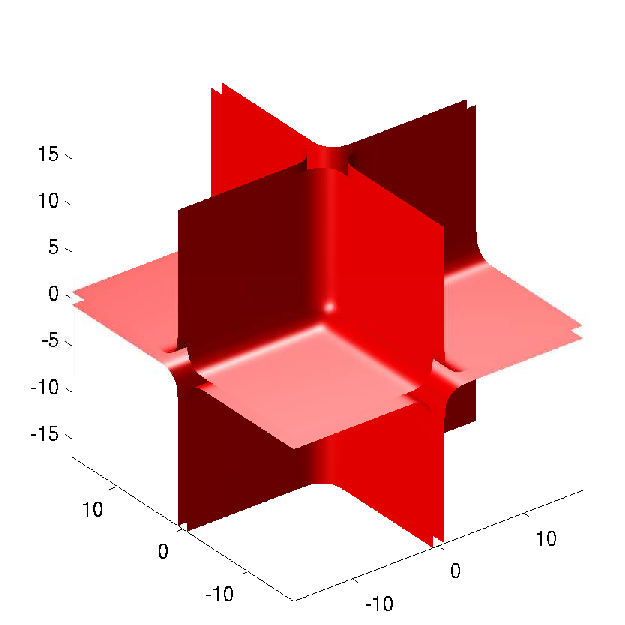
\includegraphics[trim=1em 0em 1em 0em, clip, width=0.25\textwidth]{\additivefigsdir/3d-kernel/3d_add_kernel_1} &
\hspace{-0.2in} 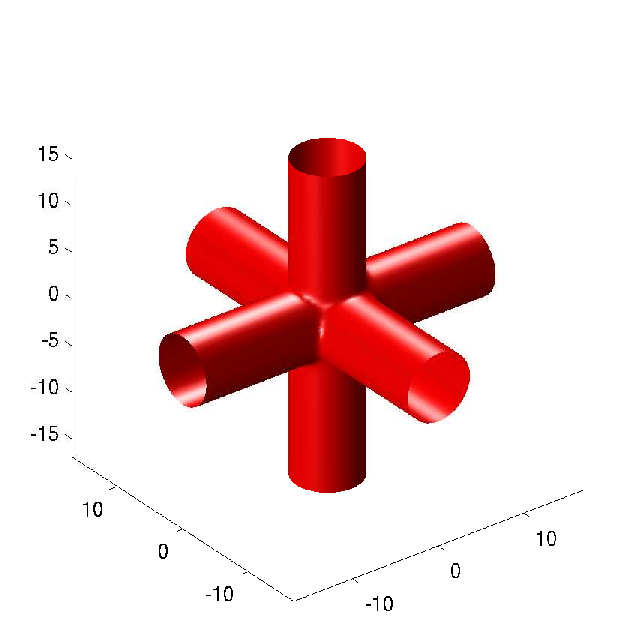
\includegraphics[trim=1em 0em 1em 0em, clip, width=0.25\textwidth]{\additivefigsdir/3d-kernel/3d_add_kernel_2} &
\hspace{-0.2in} 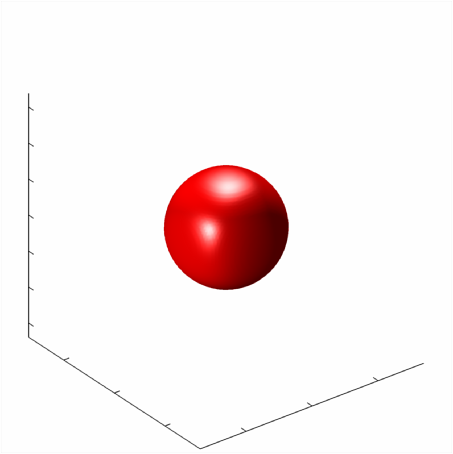
\includegraphics[trim=1em 0em 1em 0em, clip, width=0.25\textwidth]{\additivefigsdir/3d-kernel/3d_add_kernel_3} & 
\hspace{-0.2in} 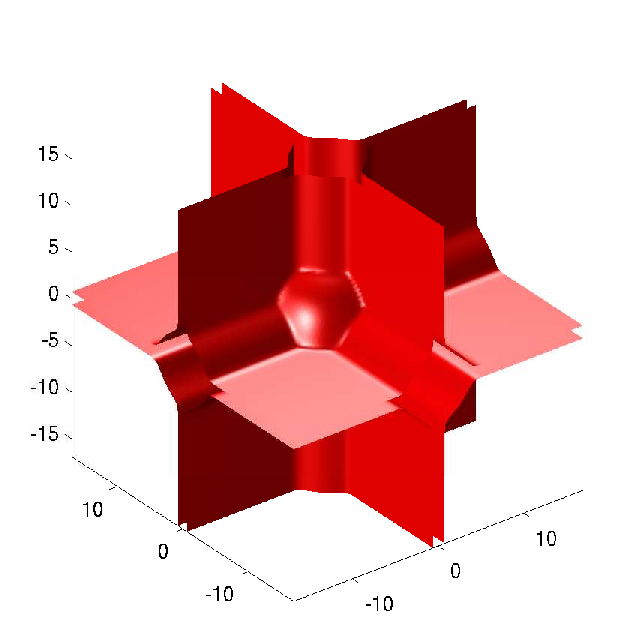
\includegraphics[trim=1em 0em 1em 0em, clip, width=0.25\textwidth]{\additivefigsdir/3d-kernel/3d_add_kernel_321}\\
1st-order terms &
2nd-order terms & 
3rd-order terms & 
All interactions \\
$k_1 + k_2 + k_3$ & $k_1k_2 + k_2k_3 + k_1k_3$ & $k_1k_2k_3$ & \\
& & Squared-exp kernel & Additive kernel\\
\end{tabular}
\caption[Isocontours of additive kernels in 3 dimensions]
{Isocontours of additive kernels in 3 dimensions.
The third-order kernel only considers nearby points relevant, while the lower-order kernels allow the output to depend on distant points, as long as they share one or more input value.}
\label{fig:kernels3d}
\end{figure}

Additive kernels have a more complex structure, and allow extrapolation far from the training data.
For example, additive kernels of the second order give high covariance between function values at points which are similar in any two input dimensions.
\Cref{fig:kernels3d} provides a geometric comparison between squared-exponential kernels and additive kernels in 3 dimensions.
\Cref{sec:additivity-multiple-dimensions} contains an example of how additive kernels extrapolate differently than local kernels.
%This is one possible reason why low-order interactions might improve predictive accuracy.




\section{Dropout in Gaussian processes}
\label{sec:dropout-gps}

\emph{Dropout} is a method for regularizing neural networks~\citep{hinton2012improving, srivastava2013improving}.
Training with dropout entails randomly and independently setting to zero (``dropping'') some proportion $p$ of features or inputs, in order to improve the robustness of the resulting network by reducing co-dependence between neurons.
To maintain similar overall activation levels, weights are multiplied by $\nicefrac{1}{p}$ at test time. Alternatively, feature activations are multiplied by $\nicefrac{1}{p}$ during training.
Test-time predictions are made by approximately averaging over all possible ways of dropping out neurons.

\citet{baldi2013understanding} and \citet{wang2013fast} analyzed dropout in terms of the effective prior induced by this procedure in several models, such as linear and logistic regression.
In this section, we perform a similar analysis for \gp{}s, examining the priors on functions that result from performing dropout in the one-hidden-layer neural network implicitly defined by a \gp{}.

Recall from \cref{sec:relating} that \gp{}s can be derived as an infinitely-wide one-layer neural network, with fixed activation functions $\feat(\vx)$ (where $k(\vx, \vx') = \feat(\vx)\tra\feat(\vx'$)), and independent random weights $\valpha$ with finite variance $\sigma^2_{\valpha}$:
%
\begin{align}
& f(\vx) = \frac{1}{K}{\mathbf \vnetweights}\tra \hPhi(\vx) = \frac{1}{K} \sum_{i=1}^K \netweights_i \hphi_i(\vx)
\\
\implies & f \distas{K \to \infty} \GPt{\expectargs{}{\valpha}\tra \feat(\vx)}{\sigma^2_{\valpha} \feat(\vx)\tra\feat(\vx')}
\label{eq:one-layer-gp-two}
\end{align}
%
Mercer's theorem implies that we can write any \gp{} prior equivalently in this way.
Having expressed a \gp{} as a neural network, we can examine the prior we get from performing dropout in this network.

This result does not hold in neural networks having a finite number of hidden features with Gaussian-distributed weights, another model class that gives rise to \gp{}s.



\subsection{Dropout on hidden layers}

First, we will examine the prior we get from independently dropping features from $\hPhi(\vx)$ by setting some of the weights $\valpha$ to zero with probability $p$.
For simplicity, we assume that $\expectargs{}{\valpha} = \vzero$.
If the weights initially have finite variance $\sigma^2_{\alpha}$ before dropout, then after dropout they'll have variance
%$\expectargs{}{ \alpha_i} = \vzero, 
%\varianceargs{}{\alpha_i} = \sigma^2$,
%then the distribution of weights after each one has been dropped out with probability $p$ is:
%
\begin{align}
r_i \simiid \textnormal{Ber}(p) \qquad %\expectargs{}{ r_i \alpha_i} = p\mu, \quad 
\varianceargs{}{r_i \alpha_i} = p \sigma_{\alpha}^2 \;.
\end{align}
%
Because \cref{eq:one-layer-gp-two} is a result of the central limit theorem, it does not depend on the form of the distribution on $\valpha$, only its mean and variance.
Thus, dropping out features of an infinitely-wide \MLP{} does not change the model at all, except to rescale the output variance.
%If we were to rescale the weights by a factor other than $p^{-1/2}$, we would only rescale the output variance of the model, leaving all other aspects identical.
%Is there a better way to drop out features that would lead to robustness?
Indeed, multiplying all weights by $p^{-1/2}$ restores the initial variance:
%
\begin{align}
%\expectargs{}{ \frac{1}{p} r_i \alpha_i } = \frac{p}{p}\mu = \mu, \quad 
\varianceargs{}{ \frac{1}{p^\frac{1}{2}} r_i \alpha_i} = \frac{p}{p} \sigma_{\alpha}^2 = \sigma_{\alpha}^2 \; .
\end{align}
%
In which case dropout on the hidden units has no effect at all.
Intuitively, this is because no individual feature can have more than an infinitesimal contribution to the network output.


\subsection{Dropout on inputs gives additive covariance}

We can also perform dropout on the $D$ inputs of the \gp{}.
For simplicity, we'll consider a stationary product kernel ${k(\vx, \vx') = \prod_{d=1}^D k_d(x_d, x_d')}$ which has been normalized such that $k(\vx, \vx') = 1$, and dropout probability of $\nicefrac{1}{2}$.
In this case, the generative model can be written as:
%
\begin{align}
r_i \simiid \textnormal{Ber} \left( \frac{1}{2} \right), \quad f(\vx) | \vr \sim \GP \left( 0, \prod_{d=1}^D k_d(x_d, x_d')^{r_d} \right)
\end{align}
%
This is a mixture of \gp{}s, each depending on a different subset of the inputs:
%
\begin{align}
p \left( f(\vx) \right) = 
\sum_{\vr} p \left( f(\vx) | \vr \right) p( \vr) = 
\frac{1}{2^D} \sum_{\vr \in \{0,1\}^D}  \GP \left(f(\vx) \,\Big|\, 0, \prod_{d=1}^D k_d(x_d, x_d')^{r_d} \right)
\label{eq:dropout-mixture}
\end{align}
We present two results ways to gain intuition about this model.

First, if the kernel on each dimension has the form ${k_d(x_d, x_d') = g \left( \frac{x_d - x_d'}{\lengthscale_d} \right)}$, as does the \kSE{} kernel, then any input dimension can be dropped out by setting its lengthscale $\lengthscale_d$ to $\infty$.
Thus, performing dropout on the inputs of a \gp{} corresponds to putting independent spike-and-slab priors on the lengthscales, with each dimension's distribution independently having ``spikes'' at $w_d = \infty$ with probability mass of $\nicefrac{1}{2}$.



Another way to understand the resulting prior is to note that the dropout mixture (\cref{eq:dropout-mixture}) has the same covariance as an additive \gp{}, scaled by a factor of $2^{-D}$:
\begin{align}
%f(\vx) \sim \textnormal{\gp} \left(0, \frac{1}{2^{-2D}} \sum_{\vr \in \{0,1\}^D}  \prod_{d=1}^D k_d(x_d, x_d')^{r_d} \right)
%f(\vx) \sim \textnormal{\gp} \left(0, \frac{1}{2^{D}} \sum_{\vr \in \{0,1\}^D}  \prod_{d=1}^D k_d(x_d, x_d')^{r_d} \right)
\cov\left( \colvec{f(\vx)}{f(\vx')} \right) = \frac{1}{2^{D}} \sum_{\vr \in \{0,1\}^D}  \prod_{d=1}^D k_d(x_d, x_d')^{r_d}
\label{eq:dropout-mixture-covariance}
\end{align}
%TODO:  Make this equation more precise
%
Therefore, ignoring higher central moments, dropout on the inputs of a \gp{} can be approximated by an additive \gp{} with all orders equally weighted.
For dropout rates $p$ other than $\nicefrac{1}{2}$, the $d$ order terms will be weighted by the corresponding binomial coefficient $D \choose d$.
This suggests an interpretation of additive \gp{}s as an approximation to a mixture of models where each model only depends on a subset of the input variables.




\section{Related work}

Since additive models are a relatively natural and easy-to-analyze model class, the literature on similar model classes is extensive.
This section attemps to provide a broad overview.

\subsubsection{Previous examples of additive \sgp{}s}

Since the non-local structure capturable by additive kernels is necessarily axis-aligned, we can naturally consider that an initial transformation of the input space might allow us to recover non-axis aligned additivity in functions.
This avenue was explored by \citet{gilboa2013scaling}, who developed a linearly-transformed first-order additive \gp{} model, called projection-pursuit \gp{} regression.
They further showed that inference in this model was possible in $\mathcal{O}(N)$ time.

\citet{durrande2011additive} also examined the properties of additive \gp{}s, and proposed a layer-wise optimization strategy for kernel hyperparameters in these models.

\citet{plate1999accuracy} constructed an additive \gp{} having only first-order and $D$th-order terms.
This model is motivated by the desire to trade off the interpretability of first-order models with the flexibility of full-order models.
Our experiments show that sometimes, the intermediate degrees of interaction contribute most of the variance.

\citet{kaufman2010bayesian} used a closely related procedure called Gaussian process \ANOVA{} to perform a Bayesian analysis of meteorological data using 2nd and 3rd-order interactions.
They also introduce a weighting scheme to ensure that each order's total contribution sums to zero.
It is not clear if this weighting scheme permits the use of the Newton-Girard formula to speed computation of the Gram matrix.
%[TODO: read and mention \citep{friedman1981projection} from Hannes]


\subsubsection{Hierarchical kernel learning}

A similar model class was recently explored by \citet{DBLP:journals/corr/abs-0909-0844} called hierarchical kernel learning (\HKL{}).
%Finally, on real datasets, HKL is outperformed by the standard \SEGP{} \citep{DBLP:journals/corr/abs-0909-0844}.
\HKL{} uses a regularized optimization framework to learn a weighted sum over an exponential number of kernels which can be computed in polynomial time.
%
\begin{figure}
\centering
\begin{tabular}{c|c}
Hierarchical kernel learning & All-orders additive \gp{} \\
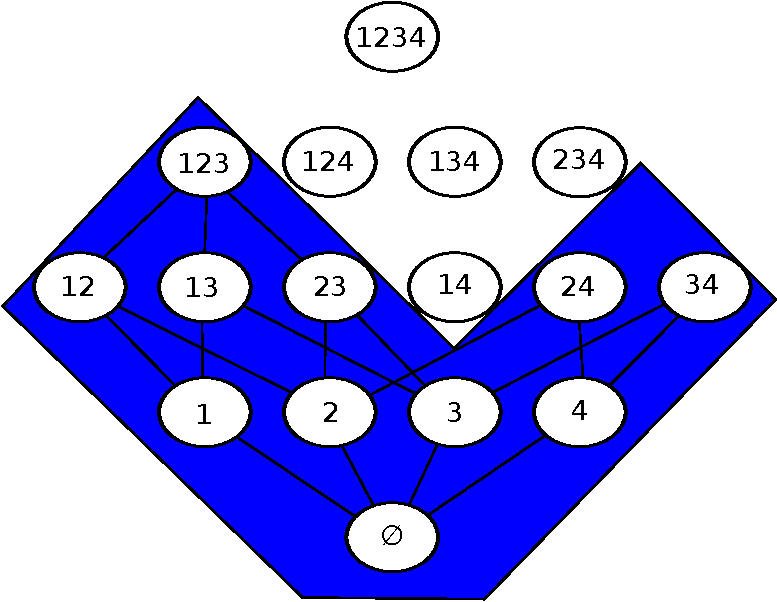
\includegraphics[height=0.35\textwidth]{\additivefigsdir/compare_models/hkl.pdf} &
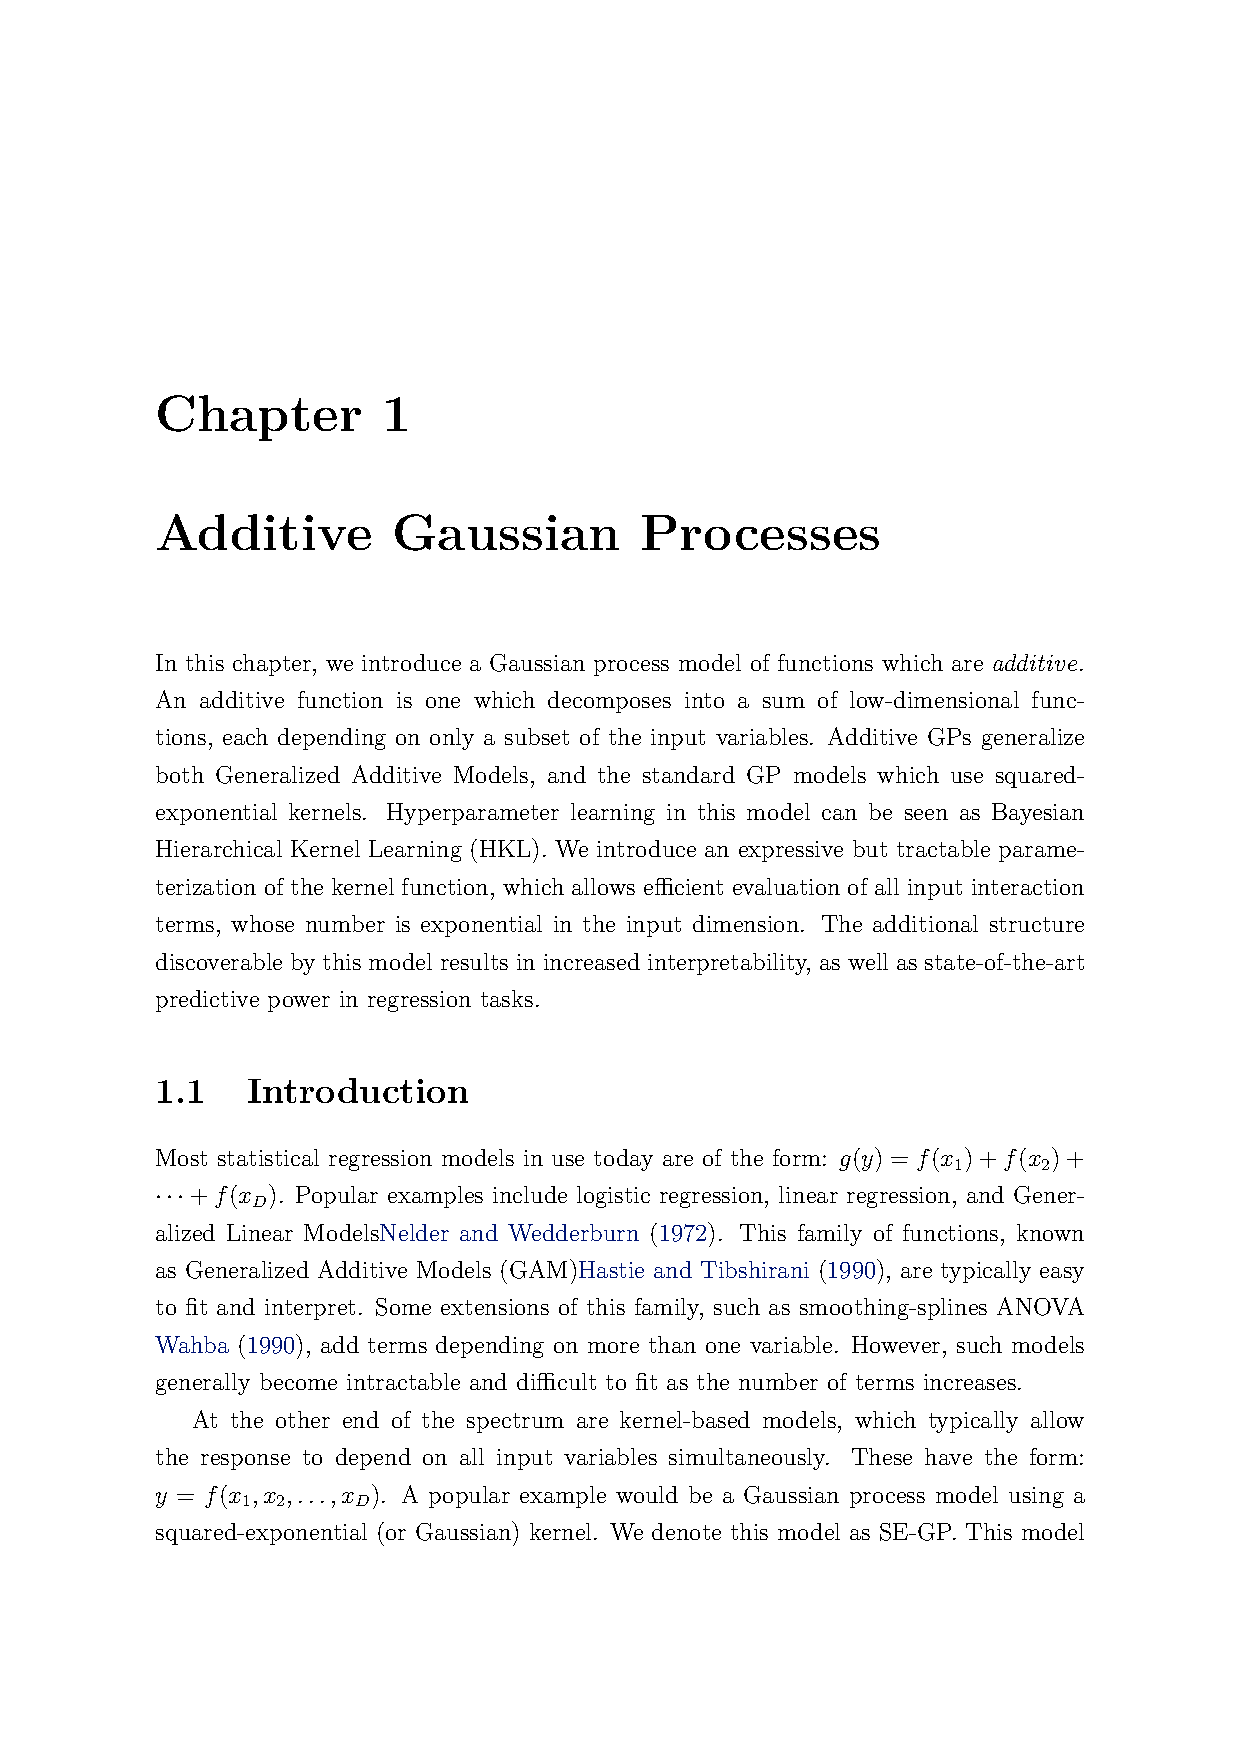
\includegraphics[height=0.35\textwidth]{\additivefigsdir/compare_models/additive.pdf}
\\ \hline \\
 Squared-exp \gp{} & First-order additive \gp{} \\
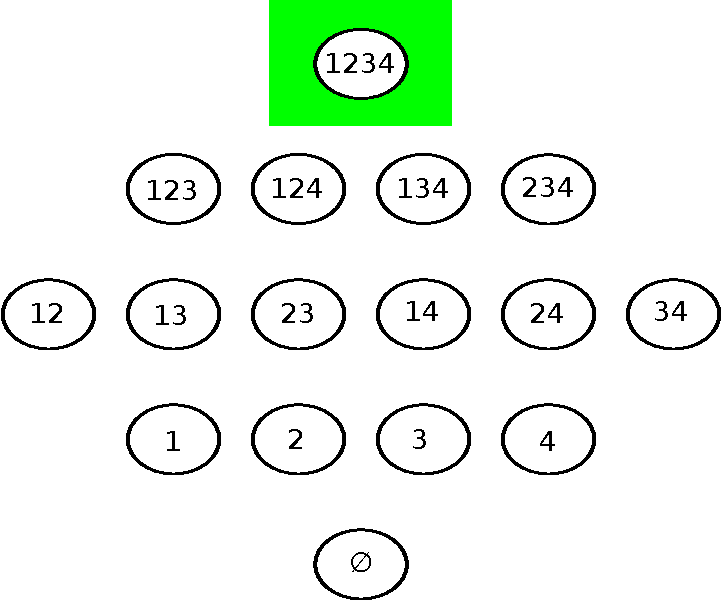
\includegraphics[height=0.35\textwidth]{\additivefigsdir/compare_models/ard.pdf} &
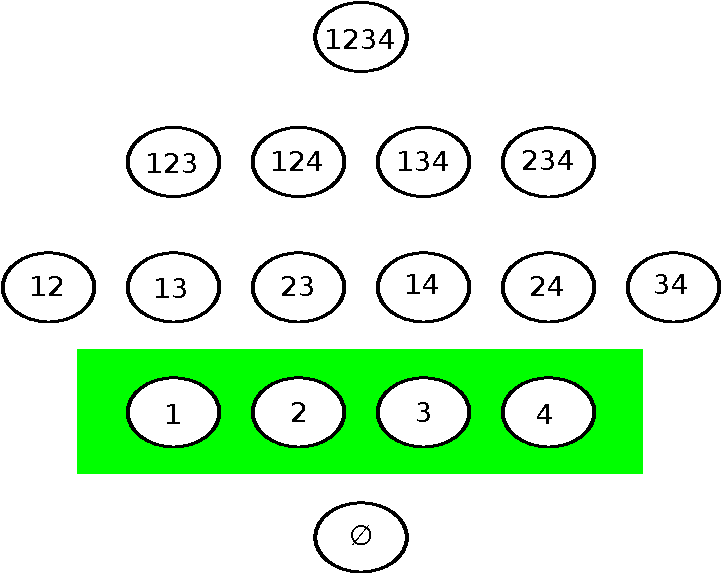
\includegraphics[height=0.35\textwidth]{\additivefigsdir/compare_models/gam.pdf} \\
\end{tabular}
\caption[A comparison of different additive model classes]
{A comparison of different additive model classes.
Nodes represent different interaction terms, ranging from first-order to fourth-order interactions.
Coloured boxes represent the weightings of different terms.
\emph{Top left: }\HKL{} can select a hull of interaction terms, but must use a pre-determined weighting over those terms.
\emph{Top right:} the additive \gp{} model can weight each order of interaction separately, but weights all terms equally within each order.
\emph{Bottom row:} The \SEGP{} and first-order additive \gp{} models are special cases of the all-orders additive \gp{}. }
\label{hulls-figure}
\end{figure}
%
This method chooses among a \emph{hull} of kernels, defined as a set of terms such that if $\prod_{j \in J} k_j(\vx, \vx')$ is included in the set, then so are all lower-order terms containing the same elements:
$\prod_{j \in J / i} k_j(\vx, \vx')$, for all $i \in J$.
\HKL{} computes the sum over all orders in $\mathcal{O}(D)$ time by the formula:
%
\begin{align}
k_a(\vx, \vx') = v^2 \prod_{d=1}^D \left(1 + \alpha k_d( x_d, x_d') \right)
\label{eqn:uniform}
\end{align}
%
which forces the weight of all $n$th order terms to be weighted by $\alpha^n$.

\Cref{hulls-figure} contrasts the \HKL{} model class with the additive \gp{} model.
Neither method is strictly more flexible than the other.
The main difficulty with this approach is that the kernel parameters are hard to set, other than by cross-validation.



\subsubsection{Support vector machines}

\citet{vapnik1998statistical} introduced the support vector \ANOVA{} decomposition, which has the same form as our additive kernel.
They recommend approximating the sum over all interactions with only one of the $D$ sets of interactions ``of appropriate order'', presumably because of the difficulty of setting the parameters of an \SVM{}.
This is an example of a model choice which can be automated in the \gp{} framework.

\citet{stitson1999support} performed experiments which favourably compared the predictive accuracy of the support vector \ANOVA{} decomposition against polynomial and spline kernels.
They too allowed only one order to be active, and set parameters by cross-validation.
%
%  The order of the kernel, kernel parameters, the allowable regression error $\epsilon$, and the cost hyperparameter $c$ were all set by a lengthy cross-validation process.

%\subsection{Smoothing Splines ANOVA}
\subsubsection{Other related models}

A closely related procedure from \citet{wahba1990spline} is smoothing-splines \ANOVA{} (\SSANOVA{}).
An \SSANOVA{} model is a weighted sum of splines along each dimension, plus a sum of splines over all pairs of dimensions, all triplets, etc, with each individual interaction term having a separate weighting parameter.
Because the number of terms to consider grows exponentially in the order, in practice, only terms of first and second order are usually considered.
%Learning in SS-ANOVA is usually done via penalized-maximum likelihood with a fixed sparsity hyperparameter.
%\citet{shawe2004kernel} define ANOVA kernels thusly: "The ANOVA kernel of degree d is like the all-subsets kernel except that it is restricted to subsets of the given cardinality $d$."


This more general model class, in which each interaction term is estimated separately, is known in the physical sciences as High Dimensional Model Representation (\HDMR{}).
\citet{rabitz1999general} review some properties and applications of this model class.

The main benefits of the model setup and parameterization proposed in this chapter are the ability to include all $D$ orders of interaction with differing weights, and the ability to learn kernel parameters individually per input dimension, allowing automatic relevance determination to operate.



\section{Regression and classification experiments}
\label{sec:additive-experiments}

\subsubsection{Choosing the Base Kernel}
A $D$-dimensional \kSE-\ARD{} kernel has $D$ lengthscale parameters and one output variance parameter.
An first-order additive $\kSE$ model has $D$ lengthscale parameters and one $D$ output variance parameters.
A fully-parametrized model including all orders of interaction with a separate output variance for each scale will have $3 \times D - 1$ effective parameters.
Because each additional parameter increases the tendency to overfit, %we recommend allowing only one kernel parameter per input dimension. 
%
%Since there always exists a parameterization of the additive function corresponding to the product kernel, we initialize the hyperparameter search for the additive kernel by first learning parameters for the equivalent product kernel.  This ensures that we start our search in a reasonable area of hyperparameter space.
%
in our experiments we fixed each one-dimensional kernel's output variance to be 1, and only learned the length-scale of each kernel.



\subsubsection{Methods}

We compared six different methods.
In the results tables below, \gp{} Additive refers to a \gp{} using the additive kernel with squared-exp base kernels.
For speed, we limited the maximum order of interaction to 10.
\gp{}-1st denotes an additive \gp{} model with only first-order interactions - a sum of one-dimensional kernels.
\gp{} Squared-exp is a \gp{} model with a \seard{} kernel.
\HKL{} was run using the all-subsets kernel, which corresponds to the same set of interaction terms as considered by the additive \gp{} with a squared-exp base kernel.

For all \gp{} models, we fit kernel parameters by the standard method of maximizing training-set marginal likelihood, using \LBFGS{}~\citep{nocedal1980updating} for 500 iterations, allowing five random restarts.
In addition to learning kernel parameters, we fit a constant mean function to the data.
In the classification experiments, approximate \gp{} inference was done using expectation propagation~\citep{minka2001expectation}.

For the regression experiments, we also compared against the structure search method from \cref{ch:grammar}, run up to depth 10, using the \SE{} and \RQ{} base kernel families.

\subsection{Datasets}

We compared these methods on a diverse set of regression and classification datasets from the UCI repository~\citep{UCI}.
Their size and dimension are given in \cref{table:regression-dataset-stats,table:classification-dataset-stats}:

\begin{table}[h]
\caption{Regression dataset statistics}
\label{tbl:Regression Dataset Statistics}
\begin{center}
\begin{tabular}{l | lllll}
Method & bach & concrete & pumadyn & servo & housing \\ \hline
Dimension      & 8    & 8        & 8       & 4     & 13 \\
Number of datapoints       & 200  & 500      & 512     & 167   & 506
\end{tabular}
\end{center}
\label{table:regression-dataset-stats}
\end{table}
%
\begin{table}[h]
\caption{Classification dataset statistics}
\label{tbl:Classification Dataset Statistics}
\begin{center}
\begin{tabular}{l | llllll}
Method & breast & pima & sonar & ionosphere & liver & heart\\ \hline
Dimension      & 9      & 8    & 60    & 32         & 6     & 13 \\
Number of datapoints      & 449    & 768  & 208   & 351        & 345   & 297
\end{tabular}
\end{center}
\label{table:classification-dataset-stats}
\end{table}

\subsubsection{Bach synthetic dataset}
In addition to standard UCI repository datasets, we generated a synthetic dataset following the same recipe as \citet{DBLP:journals/corr/abs-0909-0844}.
This dataset was designed to demonstrate the advantages of \HKL{} over \gp{}-\SE{}.
%From a covariance matrix drawn from a Wishart distribution with 1024 degrees of freedom, we select 8 variables.
It is generated by passing correlated Gaussian-distributed inputs $x_1, x_2, \dots, x_8$ through the quadratic function
%
\begin{align}
f(\vx) = \sum_{i=1}^4 \sum_{j=1+1}^4 x_i x_j + \epsilon \qquad \epsilon \sim \Nt{0}{\sigma_\epsilon}
\end{align}
%
%which sums all 2-way products of the first 4 variables, and adds Gaussian noise $\epsilon$.
This dataset will presumably be well-modeled by an additive kernel which includes all two-way interactions over the first 4 variables, but does not depend on the extra 4 correlated nuisance inputs or the higher-order interactions.%, as well as the higher-order interactions.
%TODO: Move description to grammar experiments?

%If the dataset is large enough, \HKL{} can construct a hull around only the 16 cross-terms optimal for predicting the output.
%\gp{}-\SE{}, in contrast, can learn to ignore the noisy copy variables, but cannot learn to ignore the higher-order interactions between dimensions.
%However, a \gp{} with an additive kernel can learn both to ignore irrelevant variables, and to ignore missing orders of interaction.
%With enough data, the marginal likelihood will favour hyperparameters specifying such a model.
%In this example, the additive \gp{} is able to recover the relevant structure.
 
 
\subsection{Results}
\Cref{tbl:Regression Mean Squared Error,tbl:Regression Negative Log Likelihood,tbl:Classification Percent Error,tbl:Classification Negative Log Likelihood} show mean performance across 10 train-test splits.
Because \HKL{} does not specify a noise model, it could not be included in the likelihood comparisons.

% --- Automatically generated by resultsToLatex2.m ---
% Exported at 19-Jan-2012 10:55:19
\begin{table}
\caption[Comparison of predictive error on regression problems]
{Regression mean squared error}
\label{tbl:Regression Mean Squared Error}
\begin{center}
\begin{tabular}{l | r r r r r}
Method & \rotatebox{0}{ bach  }  & \rotatebox{0}{ concrete  }  & \rotatebox{0}{ pumadyn-8nh }  & \rotatebox{0}{ servo }  & \rotatebox{0}{ housing }  \\ \hline
Linear Regression & $1.031$ & $0.404$ & $0.641$ & $0.523$ & $0.289$ \\
\gp{}-1st & $1.259$ & $0.149$ & $0.598$ & $0.281$ & $0.161$ \\
\HKL{} & $\mathbf{0.199}$ & $0.147$ & $0.346$ & $0.199$ & $0.151$ \\
\gp{} Squared-exp & $\mathbf{0.045}$ & $0.157$ & $0.317$ & $0.126$ & $\mathbf{0.092}$ \\
\gp{} Additive & $\mathbf{0.045}$ & $\mathbf{0.089}$ & $\mathbf{0.316}$ & $\mathbf{0.110}$ & $0.102$ \\
Structure Search & $\mathbf{0.044}$ & $\mathbf{0.087}$ & $\mathbf{0.315}$ & $\mathbf{0.102}$ & $\mathbf{0.082}$
\end{tabular}
\end{center}
%\end{table}
% End automatically generated LaTeX
%
% --- Automatically generated by resultsToLatex2.m ---
% Exported at 19-Jan-2012 10:55:19
%\begin{table}[h!]
\caption[Comparison of predictive likelihood on regression problems]
{Regression negative log-likelihood}
\label{tbl:Regression Negative Log Likelihood}
\begin{center}
\begin{tabular}{l | r r r r r}
Method & \rotatebox{0}{ bach  }  & \rotatebox{0}{ concrete  }  & \rotatebox{0}{ pumadyn-8nh }  & \rotatebox{0}{ servo }  & \rotatebox{0}{ housing }  \\ \hline
Linear Regression & $2.430$ & $1.403$ & $1.881$ & $1.678$ & $1.052$ \\
\gp{}-1st & $1.708$ & $0.467$ & $1.195$ & $0.800$ & $0.457$ \\
GP Squared-exp & $\mathbf{-0.131}$ & $0.398$ & $0.843$ & $0.429$ & $0.207$ \\
GP Additive & $\mathbf{-0.131}$ & $\mathbf{0.114}$ & $\mathbf{0.841}$ & $\mathbf{0.309}$ & $0.194$ \\
Structure Search & $\mathbf{-0.141}$ & $\mathbf{0.065}$ & $\mathbf{0.840}$ & $\mathbf{0.265}$ & $\mathbf{0.059}$
\end{tabular}
\end{center}
\end{table}
% End automatically generated LaTeX
%
% --- Automatically generated by resultsToLatex2.m ---
% Exported at 03-Jun-2011 00:23:25
\begin{table}
\caption[Comparison of predictive error on classification problems]
{Classification percent error}
\label{tbl:Classification Percent Error}
\begin{center}
\begin{tabular}{l | r r r r r r}
Method & \rotatebox{0}{ breast }  & \rotatebox{0}{ pima }  & \rotatebox{0}{ sonar }  & \rotatebox{0}{ ionosphere }  & \rotatebox{0}{ liver }  & \rotatebox{0}{ heart }  \\ \hline
Logistic Regression & $7.611$ & $24.392$ & $26.786$ & $16.810$ & $45.060$ & $\mathbf{16.082}$ \\
\gp{}-1st & $\mathbf{5.189}$ & $\mathbf{22.419}$ & $\mathbf{15.786}$ & $\mathbf{8.524}$ & $\mathbf{29.842}$ & $\mathbf{16.839}$ \\
\HKL{} & $\mathbf{5.377}$ & $24.261$ & $\mathbf{21.000}$ & $9.119$ & $\mathbf{27.270}$ & $\mathbf{18.975}$ \\
\gp{} Squared-exp & $\mathbf{4.734}$ & $\mathbf{23.722}$ & $\mathbf{16.357}$ & $\mathbf{6.833}$ & $\mathbf{31.237}$ & $\mathbf{20.642}$ \\
\gp{} Additive & $\mathbf{5.566}$ & $\mathbf{23.076}$ & $\mathbf{15.714}$ & $\mathbf{7.976}$ & $\mathbf{30.060}$ & $\mathbf{18.496}$ \\
\end{tabular}
\end{center}
%\end{table}
% End automatically generated LaTeX
%
% --- Automatically generated by resultsToLatex2.m ---
% Exported at 03-Jun-2011 00:23:28
%\begin{table}[h!]
\caption[Comparison of predictive likelihood on classification problems]
{Classification negative log-likelihood}
\label{tbl:Classification Negative Log Likelihood}
\begin{center}
\begin{tabular}{l | r r r r r r}
Method & \rotatebox{0}{ breast }  & \rotatebox{0}{ pima }  & \rotatebox{0}{ sonar }  & \rotatebox{0}{ ionosphere }  & \rotatebox{0}{ liver }  & \rotatebox{0}{ heart }  \\ \hline
Logistic Regression & $0.247$ & $0.560$ & $4.609$ & $0.878$ & $0.864$ & $0.575$ \\
\gp{}-1st & $\mathbf{0.163}$ & $\mathbf{0.461}$ & $\mathbf{0.377}$ & $\mathbf{0.312}$ & $\mathbf{0.569}$ & $\mathbf{0.393}$ \\
\gp{} Squared-exp & $\mathbf{0.146}$ & $0.478$ & $\mathbf{0.425}$ & $\mathbf{0.236}$ & $\mathbf{0.601}$ & $0.480$ \\
\gp{} Additive & $\mathbf{0.150}$ & $\mathbf{0.466}$ & $\mathbf{0.409}$ & $\mathbf{0.295}$ & $\mathbf{0.588}$ & $\mathbf{0.415}$ \\
\end{tabular}
\end{center}
\end{table}
% End automatically generated LaTeX

The model with best performance on each dataset is in bold, along with all other models that were not significantly different under a paired $t$-test.
%The additive model never performs significantly worse than any other model, and sometimes performs significantly better than all other models.
The additive and structure search methods usually outperformed the other methods, especially on regression problems.

%The difference between all methods is larger in the case of regression experiments.

The structure search outperforms the additive \gp{}, but at the cost of a slow search over kernels.
The additive \gp{} performed best on datasets well-explained by low orders of interaction, and approximately as well as the \SE{}-\gp{} model on datasets which were well explained by high orders of interaction (see \cref{tbl:all_orders}).
Because the additive \gp{} is a superset of both the \gp{}-1st model and the \kSE{}-\gp{} model, instances where the additive \gp{} performs slightly worse are presumably due to over-fitting, or due to the hyperparameter optimization becoming stuck in a local maximum. % Absence of over-fitting may explain the relatively strong performance of GP-GAM on classification tasks.  
Performance could be expected to benefit from approximately integrating over the kernel parameters.

The performance of \HKL{} is consistent with the results in \citet{DBLP:journals/corr/abs-0909-0844}, performing competitively but slightly worse than \SE{}-\gp{}.%  This is especially clear in the case of the regression tasks.


\subsubsection{Source code}
Additive Gaussian processes are particularly appealing in practice because their use requires only the specification of the base kernel; all other aspects of \gp{} inference remain the same.
Note that we are also free to choose a different covariance function along each dimension.

All of the experiments in this chapter were performed using the standard \GPML{} toolbox, available at \url{gaussianprocess.org/gpml/code}.
The additive kernel described in this chapter is included in the latest release.
Code to perform all experiments in this chapter is available at \url{github.com/duvenaud/additive-gps}





\section{Conclusions}

%We present a simple model which generalizes two widely-used classes of models.  A large increase in modeling power is gained at only modest computational cost.
In this chapter, we presented a tractable \gp{} model consisting of a sum of exponentially-many functions, each depending on a different subset of the inputs.
%This a simple family of models which generalizes two widely-used classes of models.
%Additive \gp{}s also introduce a tractable new type of structure into the \gp{} framework.
Our experiments indicate that, to varying degrees, such additive structure is useful for modeling real datasets.
When it is present, modeling this structure allows our model to perform better than standard \gp{} models.
In the case where no such structure exists, the higher-order interaction terms present in the kernel can recover arbitrarily flexible models, as well.
The additive \gp{} also affords some degree of interpretability: the variance parameters on each order of interaction indicate which sorts of structure are present the data.

The model class considered in this chapter is a subset of that explored by the structure search presented in \cref{ch:grammar}.
Thus additive \gp{}s can be considered a quick-and-dirty structure search, being strictly more limited in the types of structure that it can discover, but much faster and simpler to implement.

Related model classes have been previously explored, most notably smoothing-splines \ANOVA{}, and the support vector \ANOVA{} decomposition.
However, these models are difficult to apply in practice because kernel parameters, regularization penalties, and the relevant orders of interaction must all be set by hand or by cross-validation.
This chapter illustrates that the \gp{} framework allows these model choices to be performed automatically.


\outbpdocument{
\bibliographystyle{plainnat}
\bibliography{references.bib}
}





%\section{Discussion}
%% --- Automatically generated by hypers_to_latex.m ---
% Exported at 12-May-2011 16:56:21
\begin{table}[h]
\caption{{\small
Hyperparameters for housing dataset
}}
\label{tbl:housing}
\begin{center}
\begin{tabular}{l | r r r r r r r r r r r r r}
Variable: & $x_1$  & $x_2$  & $x_3$  & $x_4$  & $x_5$  & $x_6$  & $x_7$  & $x_8$  & $x_9$  & $x_10$  & $x_11$  & $x_12$  & $x_13$  \\ \hline
ARD Lengthscale & $1508.26$  & $504.64$  & $296.62$  & $3.91$  & $0.08$  & $2.21$  & $5.77$  & $2.77$  & $424.77$  & $0.74$  & $233.78$  & $605.23$  & $3.75$  \\ 
\hline
ADD Lengthscale & $392.41$  & $147.62$  & $183.48$  & $12.16$  & $0.04$  & $2.33$  & $5.71$  & $0.49$  & $402.78$  & $0.68$  & $322.01$  & $1027.36$  & $1.48$  \\
ADD Variance & $0.29$ & $0.29$ & $0.29$ & $0.44$ & $0.02$ & $19.14$ & $0.25$ & $0.97$ & $0.29$ & $10.77$ & $0.29$ & $0.29$ & $0.37$ \\ \hline
Order of Interaction: & \nth{1} & \nth{2} & \nth{3} & \nth{4} & \nth{5} & \nth{6} & \nth{7} & \nth{8} & \nth{9} & \nth{10} \\
ADD Order Variance & $0.1$\% & $0.1$\% & $0.1$\% & $0.0$\% & $0.0$\% & $0.0$\% & $0.0$\% & $0.0$\% & $0.0$\% & $99.8$\% \\ \hline
\end{tabular}
\end{center}
\end{table}
% End automatically generated LaTeX

%% --- Automatically generated by hypers_to_latex.m ---
% Exported at 12-May-2011 16:56:20
\begin{table}[h]
\caption{{\small
Hyperparameters for pima dataset
}}
\label{tbl:pima}
\begin{center}
\begin{tabular}{l | r r r r r r r r}
Variable: & $x_1$  & $x_2$  & $x_3$  & $x_4$  & $x_5$  & $x_6$  & $x_7$  & $x_8$  \\ \hline
ARD Lengthscale & $0.30$  & $0.05$  & $4.15$  & $3.62$  & $0.26$  & $1.78$  & $326.52$  & $0.76$  \\ 
\hline
ADD Lengthscale & $0.23$  & $0.05$  & $3.75$  & $6.37$  & $0.27$  & $1.81$  & $107.98$  & $0.58$  \\
ADD Variance & $2.47$ & $0.03$ & $0.86$ & $0.75$ & $0.35$ & $1.56$ & $0.71$ & $60.36$ \\ \hline
Order of Interaction: & \nth{1} & \nth{2} & \nth{3} & \nth{4} & \nth{5} & \nth{6} & \nth{7} & \nth{8} \\
ADD Order Variance & $0.0$\% & $0.1$\% & $0.1$\% & $0.3$\% & $0.0$\% & $29.0$\% & $0.1$\% & $70.4$\% \\ \hline
\end{tabular}
\end{center}
\end{table}
% End automatically generated LaTeX



%As a special case, additive kernels with only one degree of interaction can be computed in something like linear time [cite Yunus?]
 % E = elsympol(Kd(:,:,[1:j-1,j+1:D]),max(R)-1);



 
 
%\subsection{Polynomial Kernels}

%A simple variation on the all-subsets kernel would be one which includes repeated terms, of the form
%\begin{equation}
%k_{h_n}({\bf x, x'}) = v_n^2 \sum_{i_1, \dots, i_n} \prod_{d=1}^n k_{i_d}(x_{i_d}, x_{i_d}') = v_n^2 \prod_{d=1}^n \sum_{i_1, \dots, i_n}^n k_{i_d}(x_{i_d}, x_{i_d}')
%\end{equation}
%This formulation allows repeated terms, such as $x_i^2$ and is equivalent to the polynomial kernel\citep{shawe2004kernel}.  However, this formulation cases the length scale of each dimension to vary with the order of interaction considered.


